\documentclass[a4paper,12pt]{article}
\usepackage[utf8]{inputenc}
\usepackage[english]{babel}
\usepackage{amsthm}
\usepackage{amsmath}
\usepackage{amssymb}
\usepackage{float}
\usepackage{enumitem}
\usepackage{url}
\usepackage[maxbibnames=99,backend=biber]{biblatex}
\usepackage{tikz}
\usepackage[english]{isodate}
\usetikzlibrary{positioning,chains,fit,shapes,calc}

\tikzset{main node/.style={circle,draw,minimum size=0.7cm,inner sep=0pt},
}

\bibliography{rel}

%amsthm setup
\newtheoremstyle{newplanestyle}%                % Name
{10pt}%                                     % Space above
{0pt}%                                     % Space below
{\itshape}%                             % Body font
{}%                                     % Indent amount
{\bfseries}%                            % Theorem head font
{.}%                                    % Punctuation after theorem head
{ }%                                     % Space after theorem head, ' ', or \newline
{\thmname{#1}\thmnumber{ #2}\thmnote{ (#3)}} % Theorem head spec (can be left empty, meaning `normal')

\newtheoremstyle{newdefinitionstyle}%                % Name
{10pt}%                                     % Space above
{0pt}%                                     % Space below
{}%                             		  % Body font
{}%                                     % Indent amount
{\bfseries}%                            % Theorem head font
{.}%                                    % Punctuation after theorem head
{ }%                                    % Space after theorem head, ' ', or \newline
{\thmname{#1}\thmnumber{ #2}\thmnote{ (#3)}} % Theorem head spec (can be left empty, meaning `normal')

\newtheoremstyle{newprovestyle}%                 % Name
{10pt}%                                 % Space above
{0pt}%                                  % Space below
{}%                             		  % Body font
{}%                                     % Indent amount
{\itshape}%                            % Theorem head font
{.}%                                    % Punctuation after theorem head
{ }%                                    % Space after theorem head, ' ', or \newline
{} % Theorem head spec (can be left empty, meaning `normal')

\theoremstyle{newplanestyle}
\newtheorem{newtheo}{Theorem}[section]
\newtheorem{newprop}[newtheo]{Proposition}
\newtheorem{newlem}[newtheo]{Lem}
\newtheorem{newcor}[newtheo]{Corollary}

\theoremstyle{newdefinitionstyle}
\newtheorem{newdef}[newtheo]{Definition}
\newtheorem{newex}[newtheo]{Example}

\theoremstyle{newprovestyle}
\newtheorem*{newprove}{Prove}


%opening
\title{A modelization of some graph isomorphism problems using constraint programming}
\author{Gianmarco Calbi}
\date{February 15, 2018}

\begin{document}
\maketitle
\cleardoublepage

\tableofcontents
\cleardoublepage

\begin{abstract}
	We will provide a modelling of some problems about isomorphism of graphs by using constraint programming. The followings are the problems that will be discussed in this paper:
	\begin{itemize}[noitemsep]
		\item \textbf{isomorphism of graphs};
		\item \textbf{isomorphism of subgraphs};
		\item \textbf{maximum common subgraph}.
	\end{itemize}
	We will starting by proving important definitions, formalisms and references to other fundamental papers, then we will deal with each of these three problems: firstly by giving its formal definition with regard to graph theory, then by explaining an intuitive idea on how to formulate and solve it, and last but not least by modelling it in terms of constraint programming.
\end{abstract}

\cleardoublepage

\section{Basic definitions}

\begin{newdef}[Graph]
	A \textit{graph} $G$ is an ordered pair $(V,E)$ such that $V$ is a finite set of vertices and $E \subseteq V \times V$ (i.e. $E = \{(u,w) : u \in V, w \in V\}$) is a finite set of edges.
\end{newdef}

\begin{newdef}[Constraint satisfaction problem]
	A finite \textit{constraint satisfaction problem} (CSP) $\mathcal{P}$ is a triple $(X, \mathcal{D}, \mathcal{C})$ where:
	\begin{itemize}[noitemsep]
		\item $X = \{x_1, x_2, \dots, x_n\}$ is a finite set of variables;
		\item $\mathcal{D} = \{D(x) : x \in X\}$ is the set of domains of variables $x$;
		\item $\mathcal{C}$ is a set of constraints between variables of $X$. 
	\end{itemize}
\end{newdef}

\noindent
Furthermore below we recall some useful formalism from \cite{Regin:1996:GAC:1892875.1892906}:
\begin{itemize}
	\item a constraint $C$ is defined on a set of variables $X(C) = \{x_i, \dots, x_j\} \subseteq X$ by a subset of the Cartesian product $D(x_i) \times \dots \times D(x_j)$ (i.e. a set of tuple denoted by $T(C)$). Later, rather than referring a constraint as $C$, we will often deal with it from a set-theory point of view by using $T(C)$;
	\item $D(C) = \bigcup_{x \in X(C)} D(x)$ is the union of domains of variables involved in constraint $C$;
	\item $k=|X(C)|$ denotes the arity of C;
	\item $\#(a,P)$ is equal to the amount of times the value $a$ occurs in tuple $P$.
\end{itemize}

\begin{newdef}[Consistency]
	Let $\mathcal{P} = (X, \mathcal{D}, \mathcal{C})$ be a CSP, $C \in \mathcal{C}$ a constraint, $x \in X(C)$ a variable and $a \in D(x)$ a value for $x$, then:
	\begin{itemize}[noitemsep]
		\item $C$ is \textit{consistent} iff $T(C) \neq \emptyset$;
		\item $a$ is \textit{consistent with $C$} iff $\exists P \in T(C)$ such that $x$ assumes value $a$ in $P$;
		\item $C$ is \textit{arc consistent} iff $\forall x \in X(C), \forall a \in D(x)$, $a$ is consistent with $C$;  
		\item the CSP $\mathcal{P}$ is \textit{arc consistent} iff $\forall C \in \mathcal{C}$, $C$ is arc consistent. Arc consistency is usually called \textit{generalized arc consistency} when dealing with $n$-ary constraints. 
	\end{itemize}
\end{newdef}

\begin{newdef}[Global cardinality constraint]
	A \textit{global cardinality constraint} is a constraint $C$ in which each value $a \in D(C)$ is associated with two integers $l_x \geq 0$ and $c_x \geq 0$ and also $T(C) = \{P : P \text{ is a tuple of } X(C) \text{ and } \forall a \in D(C),\ l_x \leq \#(a, P) \leq c_x \}$.
\end{newdef}

\begin{newdef}[Value graph]
	The \textit{value graph} of an \textit{n}-ary constraint $C$ is the bipartite graph $GV(C) = (X(C), D(C), E)$ where $\forall x \in X(C),\ (x,a) \in E \text{ iff } a \in D(x)$.
\end{newdef}

\paragraph*{Other notions.}
For all details about formalism refer to \cite{Regin:1996:GAC:1892875.1892906}, moreover notions about flow theory on graphs are taken for granted.

\cleardoublepage

\section{Decide graph isomorphism using CP}\label{sec-gip}
In this part we will starting by giving a definition of the graph isomorphism decision problem, then we will provide a prior intuition to frame the problem, followed by a more formal definition and last we will go beyond the requests by also indicating a reasonable strategy to solve the problem using flow methods supplied by \cite{Regin:1996:GAC:1892875.1892906}.

\begin{newdef}[Isomorphic graphs]
	Two graphs $G=(V,E)$ and $G'=(V',E')$ are \textit{isomorphic} if there exists a function $f : V \to V'$ such that $(u,v) \in E \leftrightarrow (f(u),f(v)) \in E'$. Then $f$ is called \textit{isomorphism}. Function $f$ is bijective, i.e $\forall w \in V', \exists !v \in V, f(w) = v$, in particular it is said ``edge-preserving bijection'' in accordance with the general notion of isomorphism being a structure-preserving bijection.
\end{newdef}\label{def-isomorphic-graphs}

\begin{newdef}[Graph isomorphism problem]
	Given two graphs $G=(V,E)$ and $G'=(V',E')$, is called \textit{graph isomorphism problem} (GIP) the problem of determining whether $G$ and $G'$ are isomorphic, that is to answer the question if $\exists f$ such that $f$ is an isomorphism for them.
\end{newdef}

\subsection{Intuition}
Let $G=(V,E)$ and $G'=(V',E')$ be two graphs for which we're interested in answering if they are isomorphic or not. Considered the definition given for a CSP, intuitively we would like to set such problem in order to end up either 1) in a configuration as represented in Figure \ref{fig:p1-intuitive-solution}, where each vertex of $G$ is linked with one and only one vertex of $G'$, or 2) in a configuration where there's no way to pair each vertex of $G$ with one vertex of $G'$ and vice-versa. For (1), i.e a bipartite graph $B=(V_B, E_B)$ where each vertex of G (left side) is linked to one and only one vertex of $G'$ (right side), the isomorphism function would emerge directly from $E_B$.


\definecolor{myblue}{RGB}{80,80,160}
\definecolor{mygreen}{RGB}{80,160,80}

\begin{figure}[H]
	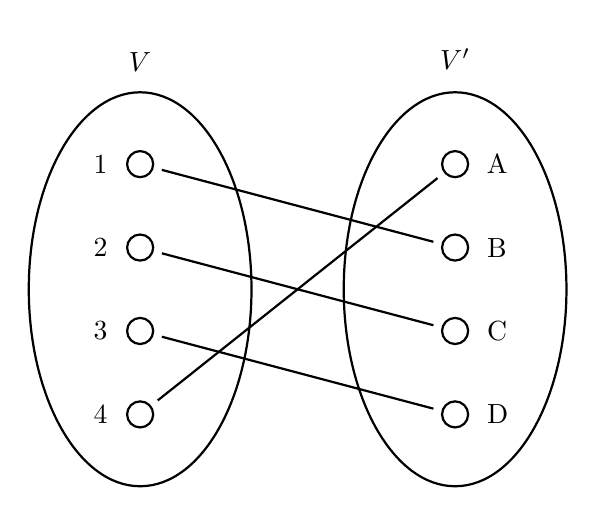
\begin{tikzpicture}[thick,
	every node/.style={draw,circle},
	fsnode/.style={fill=white},
	ssnode/.style={fill=white},
	every fit/.style={ellipse,draw,inner sep=0pt,text width=2cm},shorten >= 3pt,shorten <= 3pt
	]
	
	% the vertices of X
	\begin{scope}[start chain=going below,node distance=7mm]
	\node[fsnode,on chain] (f1) [label=left: 1] {};
	\node[fsnode,on chain] (f2) [label=left: 2] {};
	\node[fsnode,on chain] (f3) [label=left: 3] {};
	\node[fsnode,on chain] (f4) [label=left: 4] {};
	\end{scope}
	
	% the vertices of V
	\begin{scope}[xshift=4cm,start chain=going below,node distance=7mm]
	\node[ssnode,on chain] (s1) [label=right: A] {};
	\node[ssnode,on chain] (s2) [label=right: B] {};
	\node[ssnode,on chain] (s3) [label=right: C] {};
	\node[ssnode,on chain] (s4) [label=right: D] {};
	\end{scope}
	
	% the set U
	\node [black,fit=(f1) (f4),label=above:$V$] {};
	% the set V
	\node [black,fit=(s1) (s4),label=above:$V'$] {};
	
	% the edges
	\draw (s1) -- (f4);
	\draw (s2) -- (f1);
	\draw (s3) -- (f2);
	\draw (s4) -- (f3);
	\end{tikzpicture}
	\centering
	\caption{Rough bipartite graph $B$ showing GIP intuitive solution for isomorphic graphs.}\label{fig:p1-intuitive-solution}
\end{figure}

\noindent
Below is listed a draft of a \textbf{viable strategy} to follow in order to achieve a GIP's answer:
\begin{enumerate}[noitemsep]
	\item define a proper CSP for GIP;
	\item iteratively filter variables' domains by using a suitable algorithm;
	\item try to find a solution by propagate and backtrack;
	\item terminate with a positive answer upon one solution is found, otherwise answer ``no'' whether exists no solution for CSP.
\end{enumerate}

\subsubsection{About the existence of multiple isomorphisms}

\begin{minipage}{0.45\textwidth}
	\centering
	\begin{figure}[H]
		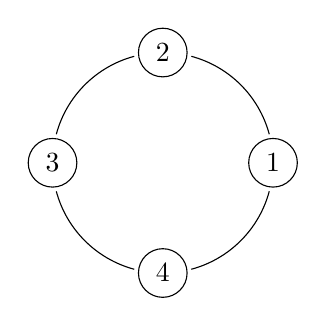
\begin{tikzpicture}
		
		\def \n {4}
		\def \radius {1.4cm}
		\def \margin {15} % margin in angles, depends on the radius
		
		\foreach \s in {1,...,\n}
		{
			\node[draw, circle] at ({360/\n * (\s - 1)}:\radius) {$\s$};
			\draw[>=latex] ({360/\n * (\s - 1)+\margin}:\radius) 
			arc ({360/\n * (\s - 1)+\margin}:{360/\n * (\s)-\margin}:\radius);
		}
		\end{tikzpicture}
		\centering
		\caption{$G=(V,E)$.}\label{fig:p1-4v-graph-rounded}
	\end{figure}
\end{minipage}\hfill
\begin{minipage}{0.45\textwidth}
	\centering
	\begin{figure}[H]
		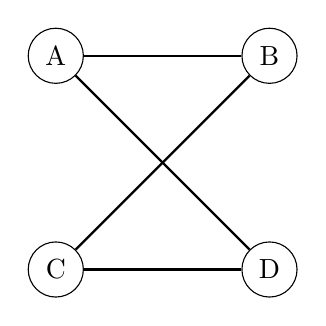
\begin{tikzpicture}
		\begin{scope}[xshift=4cm]
		\node[main node] (1) {A};
		\node[main node] (2) [right = 2cm  of 1]  {B};
		\node[main node] (3) [below = 2cm  of 1] {C};
		\node[main node] (4) [right = 2cm  of 3] {D};
		
		\path[draw,thick]
		(1) edge node {} (2)
		(1) edge node {} (4)
		(3) edge node {} (2)
		(3) edge node {} (4)
		;
		\end{scope}
		\end{tikzpicture}
		\centering
		\caption{$G'=(V',E')$.}\label{fig:p1-4v-graph-squared}
	\end{figure}
\end{minipage}

\vspace{2em}

Consider the two graphs in Figure \ref{fig:p1-4v-graph-rounded} and Figure \ref{fig:p1-4v-graph-squared}, they are clearly isomorphic, but there exists more than one isomorphism function for them. Indeed there are eight different isomorphisms $g^{(1)}$, $g^{(2)}$, $\dots$, $g^{(8)}$ for $G$ and $G'$, defined as following:
\begin{alignat*}{5}
g^{(1)} &: g^{(1)}(1) &= A, g^{(1)}(2) &= B, g^{(1)}(3) &= C, g^{(1)}(4) &= D;\\
g^{(2)} &: g^{(2)}(1) &= A, g^{(2)}(2) &= D, g^{(2)}(3) &= C, g^{(2)}(4) &= B;\\
g^{(3)} &: g^{(3)}(1) &= B, g^{(3)}(2) &= A, g^{(3)}(3) &= D, g^{(3)}(4) &= C;\\
g^{(4)} &: g^{(4)}(1) &= B, g^{(4)}(2) &= C, g^{(4)}(3) &= D, g^{(4)}(4) &= A \text{ (note\footnotemark)};\\
g^{(5)} &: g^{(5)}(1) &= C, g^{(5)}(2) &= B, g^{(5)}(3) &= A, g^{(5)}(4) &= D;\\
g^{(6)} &: g^{(6)}(1) &= C, g^{(6)}(2) &= D, g^{(6)}(3) &= A, g^{(6)}(4) &= B;\\
g^{(7)} &: g^{(7)}(1) &= D, g^{(7)}(2) &= A, g^{(7)}(3) &= B, g^{(7)}(4) &= C;\\
g^{(8)} &: g^{(8)}(1) &= D, g^{(8)}(2) &= C, g^{(8)}(3) &= B, g^{(8)}(4) &= A;
\end{alignat*}
\footnotetext{Note that the definition given here for $f$ is also the one represented in Figure \ref{fig:p1-intuitive-solution}.}
Despite the existence of multiple isomorphisms, in order to decide the isomorphism problem, we only care that at least one exists, thus finding even just one $g^{(i)}$ ($i \in \{1,\dots,8\}$) would be enough to decide that these two graphs are isomorphic. This reasoning can be extended to all graphs.

\subsection{CSP formal definition for GIP}
Given two graphs $G=(V,E)$ and $G'=(G',V')$ for which we want to decide GIP, we define a related CSP triple $\mathcal{P}=(X,\mathcal{D},\mathcal{C})$ (its elements are described in details right below).

\paragraph{Variables $X$.}
We define a variable $x_v$ for each vertex $v \in V$, that is $X = \{x_v : v \in V\}$;

\paragraph{Domains $\mathcal{D}$.}
Our aim is to end up in a situation when each vertex $v \in V$ is associated with one vertex $u \in V'$, thus $\mathcal{D}(x_v) \subseteq V'$. Moreover, since for Definition \ref{def-isomorphic-graphs} we know that an isomorphism is an edge-preserving bijection, then for any two vertices $v \in V$ and $u \in V'$, $f(v)=u \rightarrow degree(u) = degree(v)$, hence we can further reduce the set of values $v$ can assume by leaving out from $\mathcal{D}(x_v)$ all vertices $u \in V'$ such that $degree(u) \neq degree(v)$. Thus:

\[
\mathcal{D}(x_v) = \{u \in V' : degree(u) = degree(v)\}
\]
where
\[
\forall v \in V,\ degree(v) = |\{u \in V : (v,u) \in E \}|
\]

\paragraph{Constraints $\mathcal{C}$.}
Constraints are the CPS' trickiest part to define. The most straightforward way is starting from isomorphism statement: for any two vertices $u$ and $v$ in $V$, $(u,v) \in E \leftrightarrow (f(u),f(v)) \in E'$, thus, for any two variables $x_u$ and $x_v$ in $X$, if $(u,v) \in E$ then $u$ and $v$ can be associated only with two vertices $u'$ and $v'$ of $V'$ such that $(u',v') \in E'$, otherwise (whether $(u,v) \notin E$), for sure, $u$ and $v$ can be associated exclusively with two vertices of $V'$ that have no edges between them in $G'$. Formally:

\[
\mathcal{C} = \{\mathcal{C}(x_u,x_v) : x_u \in X, x_v \in X \text{ and } x_u \neq x_v\}
\]
where
\begin{equation*}
\mathcal{C}(x_u,x_v) = 
	\begin{cases}
\{(u',v') \in E' : u' \in D(x_u) \text{ and } v' \in D(x_v)\}, \hfill \text{if } (u,v) \in E \\
\{(u',v') \in D(x_u) \times D(x_v) : (u',v') \notin E' \text{ and } u' \neq v'\}, \text{ else\footnotemark}
	\end{cases}
\end{equation*}

\footnotetext{This case involves all possible values for $u'$ and $v'$ as long as there isn't an edge between them in $G'$ and obviously $u' \neq v'$.}

\subsection{Idea about solving isomorphism CSP with flow}
\cite{Regin:1996:GAC:1892875.1892906} has provided flow theory application to solve CSPs, in particular we would like to exploit Proposition 2 restated below for clarity.

\begin{newprop}\label{reg-prop}
Let $C$ be a global cardinality constraint of arity $k$ and $N(C)$ be the value network of $C$; the following two properties are equivalent:
\begin{itemize}
	\itemsep0em
	\item $C$ is consistent;
	\item there is a maximum flow from $s$ to $t$ in $N(C)$ of value $k$.
\end{itemize}
\end{newprop}

Intuitively by defining our CSP as a set of AllDiff GCC flow problems over their value networks, then filtering by applying maximum flow algorithm achieve an answer to the decision problem: 
\begin{enumerate}
	\item If we end up in a state where for each $C(x_u, x_v) \in \mathcal{C}$ there exists a maximum flow from $s_c$ to $t_c$ of value $k_c$ (for binary constraint the value of $k_c$ is always equal to 2), then, for Proposition \ref{reg-prop}, $C$ is consistent. Moreover, for AllDiff definition, for each $C$ there exists exactly one assignment $(u',v')$ that satisfy the constraint $C$, therefore $G$ and $G'$ are clearly isomorphic.
	\item Otherwise, filtering with AllDiff constraints in value networks that have a maximum flow less than $2$, force variables' domains to get empty and clearly show that $G$ and $G'$ are not isomorphic.
\end{enumerate}
\cleardoublepage

\section{Decide subgraph isomorphism problem}\label{sec-sip}
As made for GIP we will proceed by frame the problem, give an intuition and then provide a formal CSP definition for it. 

\begin{newdef}[Subgraph isomorphism problem]
	Given two graphs $G=(V,E)$ and $G'=(V',E')$. The \textit{subgraph isomorphism problem} (SIP) consists in finding a graph $G_s = (V_s, E_s)$ such that:
	\begin{enumerate}[noitemsep]
		\item $G_s$ is a subgraph of $G$, i.e. $V_s \subseteq V$ and $E_s = \{(u,v) : u \in V_s, v \in V_s \text{ and } (u,v) \in E \}$;
		\item $G_s$ and $G'$ are isomorphic.
	\end{enumerate}

\subparagraph{Nota bene.}In the following, given any two graphs $G=(V,E)$ and $G'=(V',E')$, we will always consider the SIP instance as the GIP instance for a subgraph of the first graph $G$ and the whole second graph $G'$, thus, if $G'$ is bigger with regard to the amount of vertices, then cannot exist a subgraph of $G$ that is isomorphic to $G'$.

\end{newdef}\label{def-sip}

\subsection{Intuition}
Once we have two graphs $G=(V,E)$ and $G'=(V',E')$ for which we want to decide GIP, the following cases may occur:
\begin{enumerate}
	\item $|V| < |V'|$;
	\item $|V| = |V'|$;
	\item $|V| > |V'|$;
\end{enumerate}
For case (1) an answer is achieved in constant time as explained in Definition \ref{def-sip} (\textit{nota bene}). Case (2) is the reduction of the SIP instance to a GIP one, therefore holds everything that has been said in Section \ref{sec-gip}. We will now focus on case (3).

GIP is demonstrated to be NP-Hard, so unless using an approximation, the problem is intractable with regards to time complexity. Consequently the smartest algorithm one can imagine would be as much complex as the algorithm that runs GIP on $G'$ and all subgraphs of $G$ would.

\subsection{A rough solution for SIP}
Taking into account what we just said, we will provide a \textit{time-complexity-mad} strategy to formulate and decide SIP using constraint programming.

Given any two graphs $G=(V,E)$ and $G'=(V',E')$ such that $|V| > |V'|$, let's consider the set $S$ containing all subgraphs $G_s$ of G such that $G_s$ has the same amount of vertices as $G'$, i.e. 
\[
\begin{split}
S = & \{G_s=(V_s, E_s) : V_s \subseteq V,\ |V_s| = |V'| \text{ and }\\
& \qquad E_s = \{(u,v) : u \in V_s, v \in V_s \text{ and } (u,v) \in E \}\}
\end{split}
\]
Let $n$ be the cardinality of $V$ and $m$ be the cardinality of $V'$ ($n > m$), then
\begin{equation}\label{sip-complexity}
|S| = \frac{n!}{(n-m)!m!} = \binom{n}{m} = \binom{|V|}{|V'|} = k
\end{equation}

We could formulate and solve SIP for $G$ and $G'$ by formulating and solving $k$ instances of GIP, one for each $G_s \in S$. 

Let's see $S$ as the set $\{s_1, s_2, \dots, s_k\}$ where $s_i$ is the $i$-th element of $S$, the worst case occurs when $\forall s_i \in S$, $s_i$ and $G'$ aren't isomorphic, otherwise the SIP is solved upon finding a GIP's positive answer for $s_j$ with $1 \leq j \leq k$. Whether a positive answer is achieved for a $j < k$, there's no reason why we would continue to solve the other $k - j$ GIP instances, so, the latter is the preferable situation we would like to have. Therefore one can develop an appropriate ordering for $S$ such that $\forall i,j :  i \leq j \leq k$, $s_i$ has more chance to be isomorphic to $G'$ than $s_j$ has, perhaps looking at vertices' degree or shortest paths, but here we won't go beyond this intuition. 

\cleardoublepage

\section{Maximum common subgraph}
Lets get started with two essential definitions.

\begin{newdef}[Common subgraph]
	Given two graphs $G=(V,E)$ and $G'=(V',E')$, a graph $H = (V_H, E_H)$ is a \textit{common subgraph} of $G$ and $G'$ if holds one of the following statements:
	\begin{enumerate}
		\item $H$ is a subgraph of $G$ and there exists a subgraph $H'$ of $G'$ such that $H$ and $H'$ are isomorphic;
		\item $H$ is a subgraph of $G'$ and there exists a subgraph $H'$ of $G$ such that $H$ and $H'$ are isomorphic;
	\end{enumerate}
\end{newdef}

\begin{newdef}[Common subgraph decision problem]
	Given two graphs $G=(V,E)$ and $G'=(V',E')$ and an integer $h > 0$, the \textit{common subgraph decision problem} consists in decide whether exists a graph $H = (V_H, E_H)$ such that:
	\begin{enumerate}[noitemsep]
		\item $H$ is a common subgraph of $G$ and $G'$;
		\item $|V_H| \geq h$.
	\end{enumerate}	
\end{newdef}

\begin{newdef}[Maximum common subgraph problem]
	Given two graphs $G=(V,E)$ and $G'=(V',E')$. The \textit{maximum common subgraph problem} (MSP) consists in finding a graph $H = (V_H, E_H)$ such that:
	\begin{enumerate}[noitemsep]
		\item $H$ is a common subgraph of $G$ and $G'$;
		\item $\nexists H'=(V_H', E_H')$ such that $H'$ is a common subgraph of $G$ and $G'$ and $|V_H'| > |V_H|$.
	\end{enumerate}	
\end{newdef}\label{def-msp}



\subsection{Intuition}
Given two graphs $G=(V,E)$ and $G'=(V',E')$ for which we want to solve MSP, there exist few cases with trivial solution, e.g. when one of the graph is empty, when they are exactly the same graph for definition, when they have different amount of connected components, etc. Below we will consider only cases for which solving MSP is not trivial. Since we're aware of the difficulty of this problem, we will supply a straightforward and naive way one could adopt to potentially solve an instance of MSP without caring too much about time complexity. 

\subsection{Restrict solution search space for MSP}
Let $G=(V,E)$ and $G'=(V',E')$ be two graphs such that $0 < |V'| \leq |V|$, then:
\begin{itemize}
	\item there always exists a solution for MSP since any two vertices $v \in V$ and $u \in V'$ are subgraphs of $V$ and $V'$ respectively and satisfy the isomorphism statement;
	\item moreover, if $\exists e=(u,v) \in E$ and $\exists e'=(u',v') \in E'$ then the two subgraphs $X = (\{u,v\}, \{e\})$ and $Y = (\{u',v'\}, \{e'\})$ are obviously isomorphic and as such they're a solution for MSP.  
\end{itemize}
Therefore, checking the existence of a vertex and/or an edge in both $G$ and $G'$ could help to reduce the overall time needed to compute MSP.

\subsection{A naive solution for MSP}
Whereas the solution method provided for SIP is \textit{time-complexity-mad}, then the strategy we will purpose for MSP is even worse, since it require to solve much more GIP instances to achieve an answer than SIP does.
\\

Given any two graphs $G=(V,E)$ and $G'=(V',E')$ and assuming that the MSP solution is not trivial for them, let's consider the two sets $X$ and $Y$ containing all the subgraphs of $G$ and $G'$ respectively, i.e.
\[
\begin{split}
X = & \{G_x=(V_x, E_x) : V_x \subseteq V \text{ and }\\
& \qquad E_x = \{(u,v) : u \in V_x, v \in V_x \text{ and } (u,v) \in E \}\}
\end{split}
\]

\[
\begin{split}
Y = & \{G_y=(V_y, E_y) : V_y \subseteq V' \text{ and }\\
& \qquad E_y = \{(u,v) : u \in V_y, v \in V_y \text{ and } (u,v) \in E' \}\}
\end{split}
\]
Now, let $W = \{w_k\}$ be the set of pairs $w_k = (x^{(k)}, y^{(k)})$ such that:
\begin{enumerate}
	\item $x^{(k)} \in X$ and $y^{(k)} \in Y$ are subgraphs of $G$ and $G'$ respectively;
	\item $x^{(k)}$ and $y^{(k)}$ have the same number of vertices, i.e. $|V_{x^{(k)}}| = |V_{y^{(k)}}|$;
	\item $W$ is ordered so that $w_{k}$ contains sets that have a number of vertices greater than or equal to those contained in $w_{k+1}$.
\end{enumerate}
Therefore
\[
\begin{split}
W = & \{w_k = (x^{(k)}, y^{(k)}) \in X \times Y : \\
& \qquad |V_{x^{(k)}}| = |V_{y^{(k)}}| \geq |V_{x^{(k+1)}}| = |V_{y^{(k+1)}}| \text{ for any } 1 \leq k < |W| \}.
\end{split}
\]
Let $n$ be the biggest between $|V|$ and $|V'|$ and $m$ be the smallest, for $|V| \neq |V'|$; $n=m=|V|$ otherwise; i.e.
\begin{alignat*}{2}
n & = max&\{|V|, |V'|\}\\
m & = min&\{|V|, |V'|\}
\end{alignat*}
then
\begin{equation*}
|W| = \sum_{j=1}^{m} \binom{m}{j} \binom{n}{j}.
\end{equation*}

We could formulate and solve MSP for $G$ and $G'$ by formulating and solving $|W|$ instances of GIP, one for each pair $w_k = (x^{(k)}, y^{(k)}) \in W$. Note that as soon as for a certain $1 \leq i < |W|$ one discovers that $x^{(i)}$ and $y^{(i)}$ are isomorphic, there's no need to go on and solve GIP for others $w_j$ with $i < j \leq |M|$ since the answer for MSP has been already achieved by assessing isomorphism for $w_i$.
\\
\\
\noindent
Since

\begin{equation*}
\sum_{j=1}^{m} \binom{m}{j} \binom{n}{j} \gg \binom{n}{m},
\end{equation*}
emerges clearly why the complexity of solving MSP is far worse than the one of solving SIP (Equation \ref{sip-complexity}) which is however known to be NP-Hard.

\cleardoublepage

\printbibliography %[heading=none]
\nocite{wiki:gip}
\nocite{wiki:msp}

\end{document}
